% --- Template for thesis / report with tktltiki2 class ---
%
% last updated 2013/02/15 for tkltiki2 v1.02

\documentclass[12pt,finnish,draft]{tktltiki2}

% tktltiki2 automatically loads babel, so you can simply
% give the language parameter (e.g. finnish, swedish, english, british) as
% a parameter for the class: \documentclass[finnish]{tktltiki2}.
% The information on title and abstract is generated automatically depending on
% the language, see below if you need to change any of these manually.
%
% Class options:
% - grading                 -- Print labels for grading information on the front page.
% - disablelastpagecounter  -- Disables the automatic generation of page number information
%                              in the abstract. See also \numberofpagesinformation{} command below.
%
% The class also respects the following options of article class:
%   10pt, 11pt, 12pt, final, draft, oneside, twoside,
%   openright, openany, onecolumn, twocolumn, leqno, fleqn
%
% The default font size is 11pt. The paper size used is A4, other sizes are not supported.
%
% rubber: module pdftex

% --- General packages ---

\usepackage[utf8]{inputenc}
\usepackage[T1]{fontenc}
\usepackage{lmodern}
\usepackage{microtype}
\usepackage{amsfonts,amsmath,amssymb,amsthm,booktabs,color,enumitem,graphicx}
\usepackage[pdftex,hidelinks]{hyperref}

\usepackage{url}
\usepackage{setspace}
\onehalfspacing

\setlength{\parskip}{1ex} % kappaleiden välinen tyhjä tila
\setlength{\parindent}{0pt} % kappaleen alun sisennys

% Automatically set the PDF metadata fields
\makeatletter
\AtBeginDocument{\hypersetup{pdftitle = {\@title}, pdfauthor = {\@author}}}
\makeatother

% --- Language-related settings ---
%
% these should be modified according to your language

% babelbib for non-english bibliography using bibtex
\usepackage[fixlanguage]{babelbib}
\selectbiblanguage{finnish}

% add bibliography to the table of contents
\usepackage[nottoc]{tocbibind}
% tocbibind renames the bibliography, use the following to change it back
\settocbibname{Lähteet}

% --- Theorem environment definitions ---

\newtheorem{lau}{Lause}
\newtheorem{lem}[lau]{Lemma}
\newtheorem{kor}[lau]{Korollaari}

\theoremstyle{definition}
\newtheorem{maar}[lau]{Määritelmä}
\newtheorem{ong}{Ongelma}
\newtheorem{alg}[lau]{Algoritmi}
\newtheorem{esim}[lau]{Esimerkki}

\theoremstyle{remark}
\newtheorem*{huom}{Huomautus}


% --- tktltiki2 options ---
%
% The following commands define the information used to generate title and
% abstract pages. The following entries should be always specified:

\title{Normalisoitu pakkausetäisyys: sovelluksia ja variaatioita}
\author{Timo Sand}
\date{\today}
\level{Kandidaatintutkielma}
\abstract{Tähän tulee tutkielman tiivistelmä} % TODO: Tiivistelmä

% The following can be used to specify keywords and classification of the paper:

\keywords{Samankaltaisuus}

% classification according to ACM Computing Classification System (http://www.acm.org/about/class/)
% This is probably mostly relevant for computer scientists
% uncomment the following; contents of \classification will be printed under the abstract with a title
% "ACM Computing Classification System (CCS):"
\classification{\textbf{Information systems - Similarity measures} \\ \textit{Theory of computation - Unsupervised learning and clustering} \\ Data mining - Clustering}

% If the automatic page number counting is not working as desired in your case,
% uncomment the following to manually set the number of pages displayed in the abstract page:
%
% \numberofpagesinformation{16 sivua + 10 sivua liitteissä}
%
% If you are not a computer scientist, you will want to uncomment the following by hand and specify
% your department, faculty and subject by hand:
%
% \faculty{Matemaattis-luonnontieteellinen}
% \department{Tietojenkäsittelytieteen laitos}
% \subject{Tietojenkäsittelytiede}
%
% If you are not from the University of Helsinki, then you will most likely want to set these also:
%
% \university{Helsingin Yliopisto}
% \universitylong{HELSINGIN YLIOPISTO --- HELSINGFORS UNIVERSITET --- UNIVERSITY OF HELSINKI} % displayed on the top of the abstract page
% \city{Helsinki}
%

\newcommand{\engl}[1]{\emph{(engl. #1)}}
\newcommand{\kolmogorov}{Kolmogorov-kompleksisuus}


\begin{document}

% --- Front matter ---

\frontmatter      % roman page numbering for front matter

\maketitle        % title page
\makeabstract     % abstract page

\tableofcontents  % table of contents

% --- Main matter ---

\mainmatter       % clear page, start arabic page numbering

\section{Johdanto} % (fold)
\label{sec:johdanto}
\iffalse
  TODO:

\fi
\label{par:intro-1}
  Kaikki data on luotu samanveroiseksi, mutta jotkut datat ovat samankaltaisempia kuin toiset.
  Esitämme tavan, jolla ilmaista tämä samankaltaisuus, käyttäen Cilibrasin ja Vitanyin esittelemää samankaltaisuuden metriikkaa \engl{similarity metric}, joka perustuu tiedoston pakkaamiseen. \cite{CV05}
  Metriikka on parametriton, eli se ei käytä datan ominaisuuksia tai taustatietoja, ja sitä voi soveltaa eri aloihin ilman muunnoksia.
  Metriikka on universaali siten, että se approksimoi parametrin, joka ilmaisee parin hallitsevan piirteen samankaltaisuutta pareittain vertailuissa.
  Se on vakaa siinä mielessä, että sen tulokset ovat riippumattomia käytetystä pakkaajasta \cite{CV05}. Pakkaajalla tarkoitetaan pakkausohjelmaa kuten \emph{gzip, ppmz, bzip2}.

  \label{par:intro-2}
  Pakkaukseen perustuva samankaltaisuus \engl{Compression-Based Similarity} on universaali metriikka, jonka kehittivät Cilibrasi ja Vitanyi \cite{CV05}.
  Yksinkertaistettuna tämä tarkoitta, että kaksi objektia ovat lähellä toisiaan, jos voimme ``pakata'' yhden objektin huomattavasti tiiviimmin toisen objektin datalla.
  Abstraktina ideana toimii se, että voimme kuvailla ytimekkäämmin yhden objektin toisen avulla, mikäli objektit ovat samankaltaisia.
  Tämän esittelemme luvussa \ref{sec:normalisoitu_pakkauset_isyys} ja samalla käymme läpi, mihin teoriaan algoritmi perustuu sekä miten se toimii.
  Edellä mainitun vakauden esittämiseen voimme käyttää useaa tosielämän pakkausalgoritmiä: tilastollista (PPMZ), Lempel-Ziv -algoritmiin pohjautuvaa hakemistollista (gzip), lohkoperusteista (bzip2) tai erityistarkoitusta varten (Gencompress).

  Kaikissa kohdissa  operoimme $O(log n)$ tarkkuudella, joka on hinta siitä että siirrytään Kolmogorv-kompleksisuudesta laskettavaan approksimaatioo

  Tarkoituksemme on koota yhteen samankaltaisuuden metriikkaan kaikki tehokkaat etäisyydet \engl{effective distances}: tehokkaat versiot Hammingin etäisyydestä, Euklidisestä etäisyydestä, Lempel-Ziv etäisyydestä ja niin edelleen.
  Tämän metriikan tulee olla niin yleinen, että se toimii yhtäläisesti ja samanaikaisesti kaikilla aloilla: musiikillä, tekstillä, kirjallisuudella, ohjelmilla, genomeilla, luonnollisen kielen määrityksillä.
  Sen pitäisi pystyä samanaikaisesti havaitsemaan kaikki samankaltaisuudet objektien välillä, joita muut etäisyydet havaitsevat erikseen.

  Kun määrittelemme ryhmän sallittavia etäisyyksiä \engl{admissible distances} haluamme sulkea pois epärealistiset, kuten $f(x,y) = \frac{1}{2}$ jokaiselle parille $x \neq y$.
  Saavutamme tämän rajoittamalla objektien lukumäärän annetussa etäisyydessä objektiin.
  Teemme tämän huomioimalla vain todellisia etäisyyksiä seuraavasti: Oletamme kiinnitetyn ohjelmointikielen, joka toimii tutkielman ajan viitekielenä.
  Tämä ohjelmointikieli voi olla yleinen kieli kuten LISP, Ruby tai se voi myös olla kiinitetty universaali Turingin kone. \cite{CV05,cilibrasi2007google}
  Valinnalla ei kuitenkaan ole merkitystä, sillä teoria on invariantti ohjelmointikielin muutoksille, kunhan pysytään tehdyssä valinnassa.


Jotta voimme soveltaa tätä ideaalia ja tarkkaa matemaattista teoriaa käytäntöön, pitää meidän korvata ei laskettavissa oleva Kolmogorov-kompleksisuus approximaatiolla käyttäen standardia pakkaajaa.

\label{par:intro-3}
  Luvussa \ref{sec:k_ytt_kohteet} esittelemme algoritmin käyttökohteita monelta eri alueelta.
  Aloitamme siitä, miten yleisesti \emph{Normalisoidun pakkausetäisyyden} (\emph{NCD}) avulla pystymme klusteroimaan tuloksia eri kategorioihin; miten musiikkikappaleet klusteroituvat saman artistin alle, miten kuvantunnistuksessa saamme ryhmitettyä samankaltaiset kuvat ja miten sienten genomeista saamme tarkan lajiryhmityksen.


  Luvun lopussa syvennymme musiikin, kuvantunnistuksen ja dokumenttien kategorisoinnin tuloksiin.


\label{par:intro-4}
  Luvussa \ref{sec:algoritmin_ongelmat_ja_ominaisuudet} esitellään NCD:n ominaisuuksia ja ongelmia.
  Ensiksi esitellään NCD:n kohinansietokykyä, eli katsotaan mitä tapahtuu kun lisätään vähitellen kohinaa toiseen tiedostoista, jota pakataan, ja mittaamalla samankaltaisuutta tämän jälkeen \cite{4167725}.
  Saamme nähdä miten paljon kohina vaikuttaa NCD:n laskemiin etäisyyksiin ja huonontaako se klusteroinnin tuloksia.


  Mikään algoritmi ei ole täydellinen, ja NCD-algoritmillakin on ongelmansa.
  Algoritmissa itsessään ei ole selvää heikkoutta, mutta sen käytössä on otettava pakkaajan valinta huomioon, koska monet suosituista pakkausalgoritmeista ovat optimoituja tietyn kokoisille tiedostoille.
  Niissä on niin kutsuttu ikkunakoko \engl{window size}, joka määrittelee mikä tiedostokoko on sopiva \cite{cebrian2005common}.
  Jos tiedostokoko on pienempi kuin ikkunakoko, niin pakkaus on tehokasta, mutta kun mennään siitä yli, pakkauksesta tulee huomattavasti tehottomampaa.
  Esittelemme tuloksia eri pakkausalgoritmien vertailuista ja mikä näistä algoritmeista on parhaimmaksi havaittu NCD:n kanssa käytettäväksi.


\label{par:intro-5}
  NCD ei ole ainut metriikka, jolla voidaan mitata samankaltaisuutta.
  Internettiä hyödyntäen on tehty metriikka, joka käyttää hakukoneita samankaltaisuuden tutkimiseen; tämä on nimetty Google-samankaltaisuusetäisyydeksi \engl{Google Similarity Distance}.
  Tämä toimii myös muilla hakukoneilla kuten Bing. Luvussa \ref{sec:muita_samankaltaisuuden_metriikoita} esitellemme tämän sekä muita samankaltaisuuden metriikoita.

% section johdanto (end)

\section{Normalisoitu Pakkausetäisyys} % (fold)
\label{sec:normalisoitu_pakkauset_isyys}
  \subsection{\kolmogorov} % (fold)
\label{sub:kolmogorov_kompleksisuus}

  Merkkijonon $x$ \emph{\kolmogorov} on pituus bitteinä, lyhimmästä tietokoneohjelmasta joka ilman syötettä palauttaa merkkijonon $x$; tämä merkitään $K(x)=K(x|\lambda)$, $\lambda$ esittää tyhjää syötettä.
  Lyhimmän tietokoneohjelman pituus, joka palauttaa $x$ syötteellä $y$, on \kolmogorov $x$:stä syötteellä $y$; tämä merkitään $K(x|y)$.
  Yksi tapa hahmottaa Kolmogorov-kompleksisuutta $K(x)$ on ajatella se pituutena bitteinä $x$:n tiiviimmin pakatussa muodossa, josta voidaan purkaa $x$ pakkauksenpurkuohjelmalla.

% subsection kolmogorov_kompleksisuus (end)
\subsection{Normalisoitu informaatioetäisyys} % (fold)
\label{sub:normalisoitu_informaatioet_isyys}

  Artikkelissa \cite{CV05} on esitelty \emph{informaatioetäisyys} $E(x,y)$, joka on määritelty lyhimpänä binääriohjelman pituutena, joka syötteellä $x$ laskee $y$:n ja syötteellä $y$ laskee $x$:n. Tämä lasketaan seuraavasti:

  \begin{align}
    E(x,y) &= max\{K(x|y),K(y|x)\}.
  \end{align}

  Normalisoitu versio informaatioetäisyydestä $E(x,y)$, jota kutsutaan \emph{normalisoiduksi informaatioetäisyydeksi}, on määritelty seuraavasti

  \begin{align}
    NID(x,y) &= \frac{ max\{K{(x|y)},K{(y|x)}\} }{ max \{K(x),K(y)\}}.
  \end{align}

  Tämä on paras mahdollinen \emph{samankaltaisuuden metriikka}, ja sen on osoitettu \cite{CV05} täyttävän vaatimukset etäisyyden metriikaksi.
  \emph{NID} ei kuitenkaan ole laskettava tai edes semi-laskettava, koska Turingin määritelmän mukaan \kolmogorov ei ole laskettava \cite{CV05}.
  Nimittäjän approksimointi annetulla pakkaajalla $C$ on $max \{C(x),C(y)\}$.
  Osoittajan paras approksimaatio on $max\{C(xy),C(yx)\} - \min\{C(x),C(y)\}$ \cite{CV05}.
  Kun \emph{NID} approksimoidaan oikealla pakkaajalla, saadaa tulos jota kutsutaan \emph{normalisoiduksi pakkausetäisyydeksi}.
  Tämä esitellään formaalisti myöhemmin.
% subsection normalisoitu_informaatioet_isyys (end)

\subsection{Normaali pakkaaja} % (fold)
\label{sub:normaali_pakkaaja}

  Seuraavaksi esitämme aksioomia, jotka määrittelevät laajan joukon pakkaajia ja samalla varmistavat \emph{normalisoidussa pakkausetäisyydessä} halutut ominaisuudet.
  Näihin pakkaajiin kuuluvat monet tosielämän pakkaajat.

  Pakkaaja $C$ on \emph{normaali} jos se täyttää seuraavat aksioomat:

  \label{idempotency}
  \begin{enumerate}
    \item \emph{Idempotenssi}: $C(xx) = C(x)$ ja $C(\lambda) = 0$, jossa $\lambda$ on tyhjä merkkijono,
    \item \emph{Monotonisuus}: $C(xy) \geq C(x)$,
    \item \emph{Symmetrisuus}: $C(xy) = C(yx)$ ja
    \item \emph{Distributiivisuus}: $C(xy) + C(z) \leq C(xz) + C(yz)$.
  \end{enumerate}
% subsection normaali_pakkaaja (end)

\subsection{Normalisoitu Pakkausetäisyys} % (fold)
\label{sub:normalisoitu_pakkauset_isyys}

  Jotta voimme soveltaa tätä ideaalia ja tarkkaa matemaattista teoriaa käytäntöön, pitää meidän korvata ei laskettavissa oleva Kolmogorov-kompleksisuus approximaatiolla käyttäen standardia pakkaajaa.

  Normalisoitua versiota \emph{hyväksyttävästä etäisyydestä} $E_c(x,y)$, joka on pakkaajaan $C$ pohjautuva approksimaatio normalisoidusta informaatioetäisyydestä, kutsutaan nimellä \emph{Normalisoitu Pakkausetäisyys (NCD)} \cite{CV05}.
  Tämä lasketaan seuraavasti

  \begin{align}
    NCD(x,y) &= \frac{C(xy)-min\{C(x),C(y)\}}{max\{C(x),C(y)\}}.
  \end{align}

  \emph{NCD} on funktioden joukko, joka ottaa argumenteiksi kaksi objektia (esim. tiedostoja tai Googlen hakusanoja) ja tiivistää nämä, erillisinä ja yhdistettyinä.
  Tämä funktioden joukko on parametrisoitu käytetyn pakkaajan $C$ mukaan.

  Käytännössä \emph{NCD}:n tulos on välillä $0 \leq r \leq 1+ \epsilon$, joka vastaa kahden tiedoston eroa toisistaan; mitä pienempi luku, sitä enemmän tiedostot ovat samankaltaisia.
  Tosielämässä pakkausalgoritmit eivät ole yhtä tehokkaita kuin teoreettiset mallit, joten virhemarginaali $\epsilon$ on lisätty ylärajaan.
  Suurimmalle osalle näistä algoritmeistä on epätodennäköistä että  $\epsilon > 0.1$.
% subsection normalisoitu_pakkauset_isyys (end)

  Luonnollinen tulkinta \emph{NCD}:stä, jos oletetaan $C(y) \geq C(x)$, on

  \begin{align}
    NCD(x,y) = \frac{C(xy)-C(x)}{C(y)}.
 \end{align}

  Eli etäisyys $x$:n ja $y$:n välillä on suhde $y$:n parannuksesta, kun $y$ pakataan käyttäen $x$:ää, ja $y$:n pakkauksesta yksinään; suhde ilmaistaan etäisyytenä bittien lukumääränä kummankin pakatun version välillä.

  Kun pakkaaja on normaali, niin \emph{NCD} on normalisoitu hyväksyttävä etäisyys, joka täyttää metriikan yhtälöt, eli se on samankaltaisuuden metriikka.

  Taulukossa \ref{tab:NCD-values} esitellään muutama arvo joilla NCD lasketaan ja mikä tulos näistä saadaan. Taulukon arvot saatu paperista \cite{cebrian2005common}

  \begin{table}[t]
    \centering
    \begin{tabular}{c|c|l}
      Arvot                    & Laskutoimitus      & NCD:n arvo \\ \hline
      $ C(xx) = 26, C(x) = 17$ & $\frac{26-17}{17} $ & $0.529$    \\ \hline
      $ C(xx) = 33, C(x) = 22$ & $\frac{33-22}{22} $ & $0.5$      \\ \hline
      $ C(xx) = 30, C(x) = 17$ & $\frac{30-17}{17} $ & $0.765$    \\ \hline
      $ C(xx) = 20, C(x) = 14$ & $\frac{20-14}{14} $ & $0.428$    \\ \hline
      $ C(xx) = 16, C(x) = 14$ & $\frac{16-14}{14} $ & $0.143$    \\ \hline
      $ C(xx) = 28, C(x) = 14$ & $\frac{28-14}{14} $ & $1$        \\
    \end{tabular}
    \caption{Normalisoituja pakkausetäisyyksiä eri syötteille.}
    \label{tab:NCD-values}
  \end{table}

% section normalisoitu_pakkauset_isyys (end)

\section{Käyttökohteet} % (fold)
\label{sec:k_ytt_kohteet}
  \subsection{Klusterointi} % (fold)
  \label{sub:klusterointi}
    \begin{itemize}
      \item Miten klusteroidaan
      \item Etäisyysmatriisi
    \end{itemize}
    \subsubsection{Kvartettimetodi} % (fold)
    \label{ssub:quartet_metodi}

    \begin{itemize}
      \item puun rakentaimnen etäisyysmatriisistä
      \item Puun operaatiot
      \item normalisoiti puun hyötyarvo $S(T)$
      \item Satunnaisuuden käyttö tarkistusiteraatiossa parhaan puun approksimoimiseksi
    \end{itemize}
    % subsubsection quartet_metodi (end)
    \subsubsection{Tuloksia} % (fold)
    \label{ssub:tuloksia}
      \begin{itemize}
        \item Musiikin genrepuu
        \item Musiikin pieni vertaus
        \item Musiikin keskikokoinen vertaus
        \item Musiikin suuri vertaus
      \end{itemize}

    % subsubsection tuloksia (end)
  % subsection klusterointi (end)
  \subsection{Kuvantunnnistus} % (fold)
  \label{sub:kuvantunnnistus}

  % subsection kuvantunnnistus (end)
% section k_ytt_kohteet (end)

\section{Algoritmin ongelmat ja ominaisuudet} % (fold)
\label{sec:algoritmin_ongelmat_ja_ominaisuudet}
  \subsection{Kohinansietokyky} % (fold)
  \label{sub:kohinansietokyky}

  % TODO: Kuvakäppyrä
  % TODO: Approximoi differentiaaliyhtälöllä
    Kun NCD:tä käytetään kahteen eri tiedostoon toista näistä voi pitää kohinallisena versiona ensimmäisestä.
    Kohinan lisääminen progressiivisesti tiedostoon voi tuottaa tietoa mittarista \engl{measure} itsestään.
    Tämän vastaavuuden perusteella voimme tehdä teoreettisen päätelmän odotetusta kohinan lisäämisen vaikutuksesta algoritmiin, mikä selittää miksi NCD voi saada suurempia arvoja kuin $1$ joissain tapauksissa. \cite{4167725}

    \begin{figure}[t]
      \begin{center}
        % \immediate\write18{pdfcrop img/noise-005}
        % 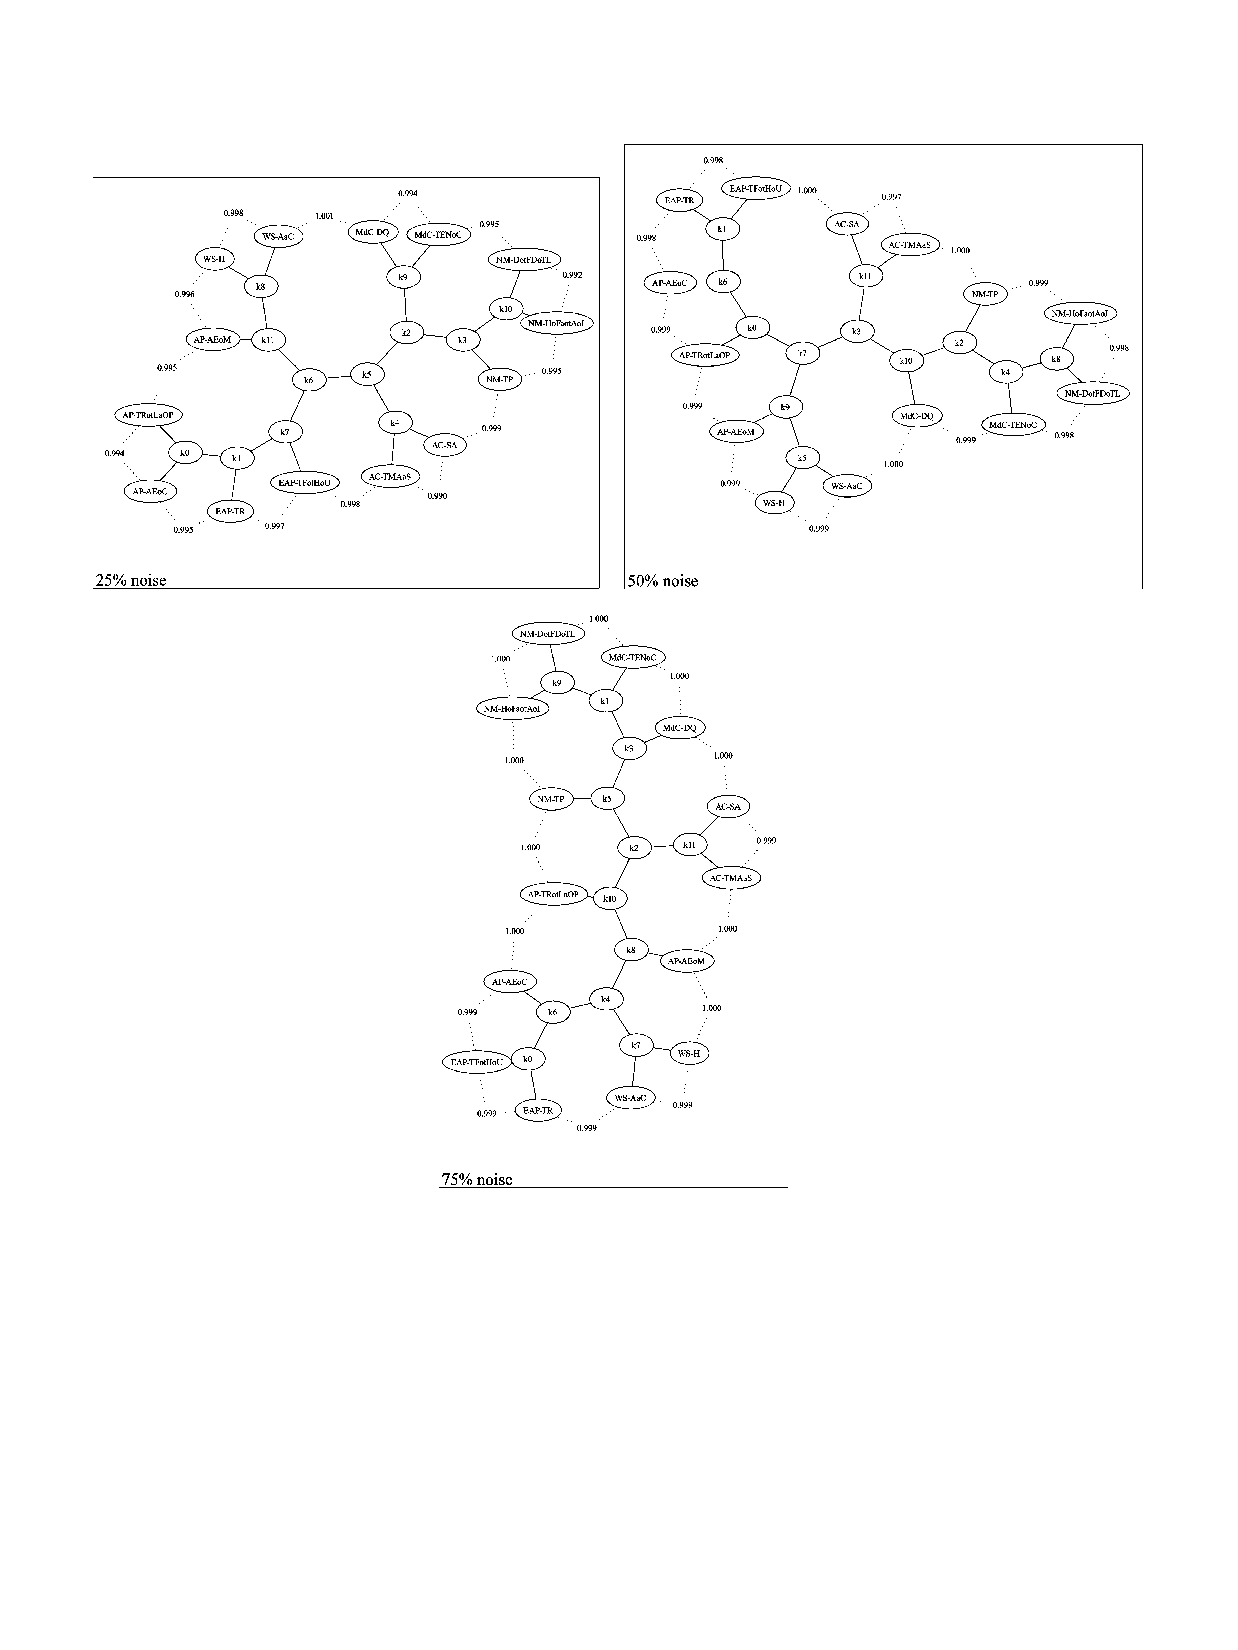
\includegraphics{img/noise-005}
      \end{center}
      \caption{Normalisoitujen pakkausetäisyyksien pohjalta klusteroituja kirjoja eri kirjoittajilta ja vaihteleva määrä kohinaa lisättynä. Merkkinnän ensimmäiset pari merkkiä ovt kirjailijan initials: AC = Agatha Christie, AP = Alexander Pope, EAP = Edgar Allan Poe, WS = William Shakespeare ja NM = Niccolo Machiavelli.
      % TODO: The quality of the clustering degrades slowly due to the linear growth of the average distortion.
      \cite{4167725}}
      \label{fig:(bzip2-best)}
    \end{figure}

  % subsection kohinansietokyky (end)

  \subsection{Pakkaajan valinta} % (fold)
  \label{sub:pakkaajan_valinta}

    \begin{figure}[t]
      \begin{center}
        \immediate\write18{pdfcrop img/bzip2-best}
          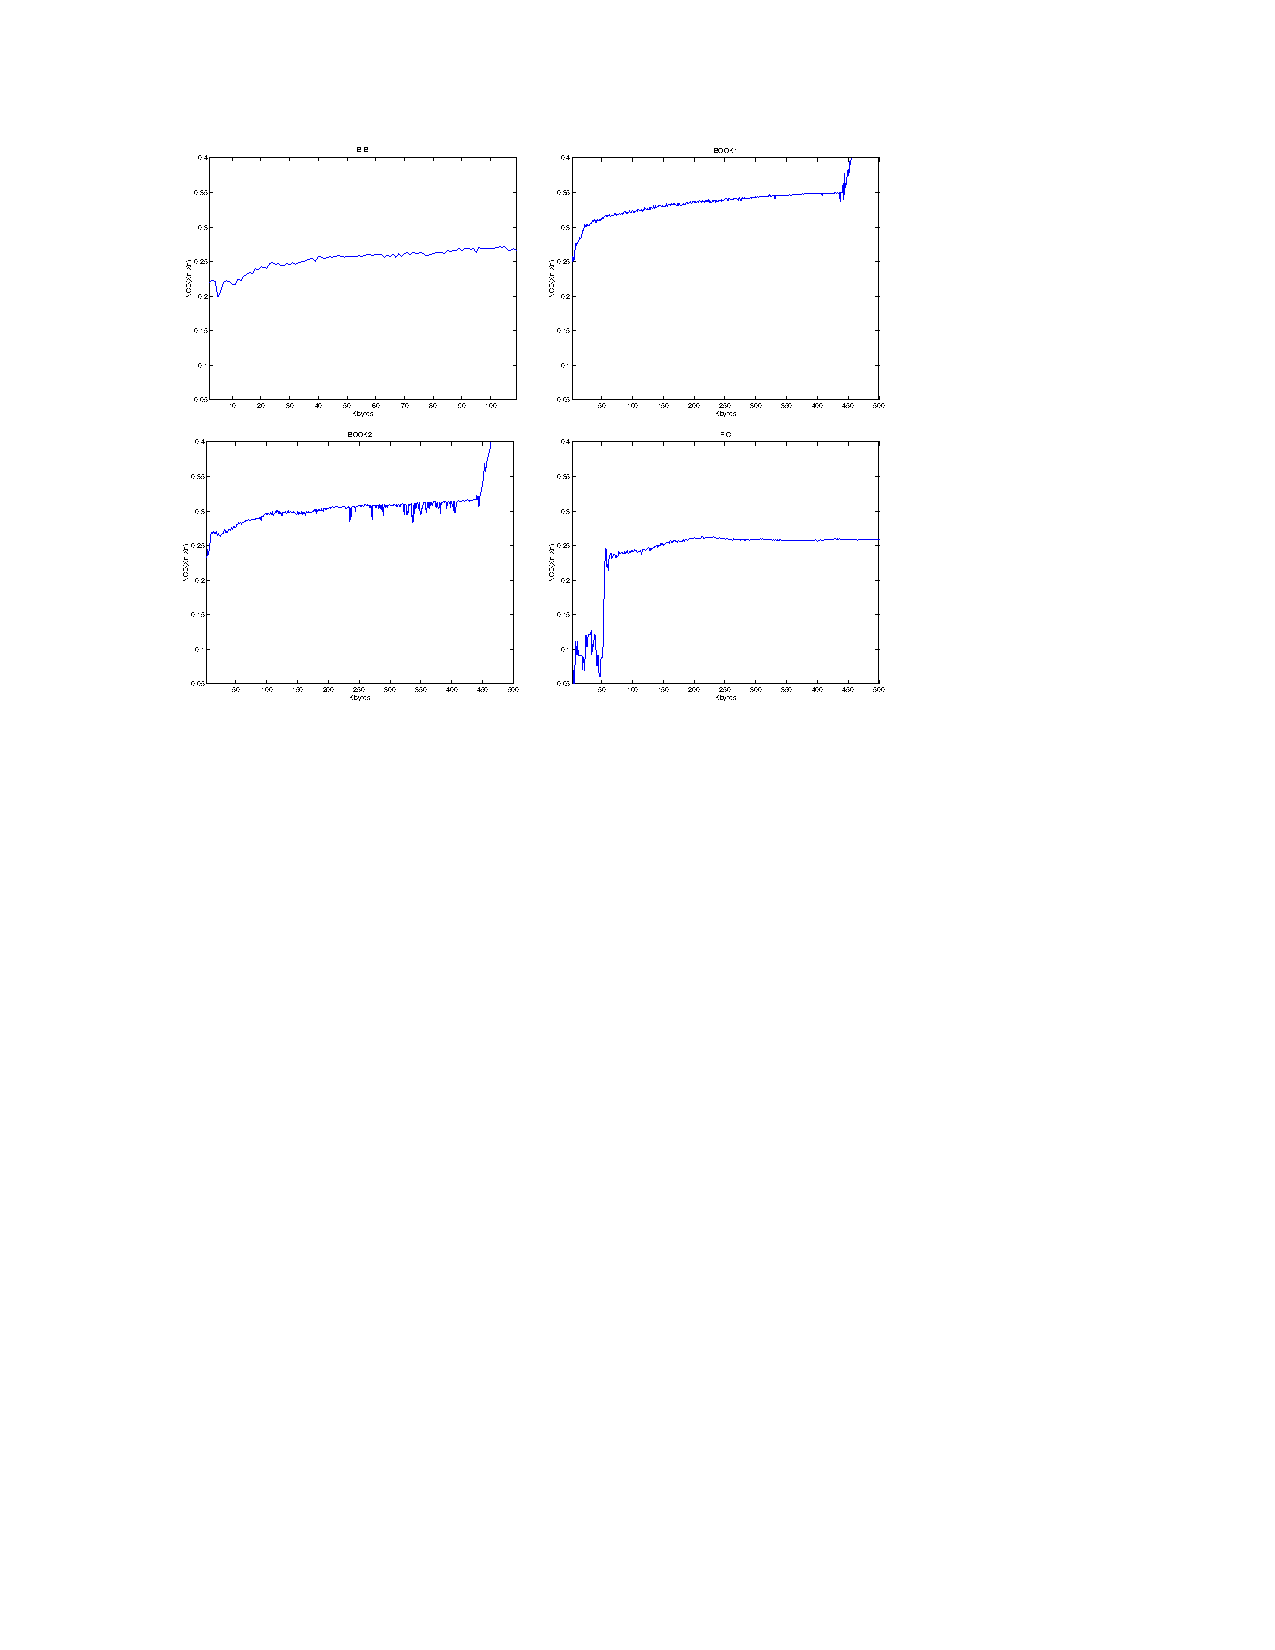
\includegraphics{img/bzip2-best}
      \end{center}
      \caption{Normalisoidut pakkausetäisyydet ensimmäisestä $n$ tavusta, neljälle tiedostolle Calgary Corpus -kokoelmasta, käyttäen \emph{bzip2} pakkaajaa asetuksella `--best' \cite{cebrian2005common}}
      \label{fig:(bzip2-best)}
    \end{figure}
    \begin{figure}[t]
      \begin{center}
        \immediate\write18{pdfcrop img/bzip2-fast}
      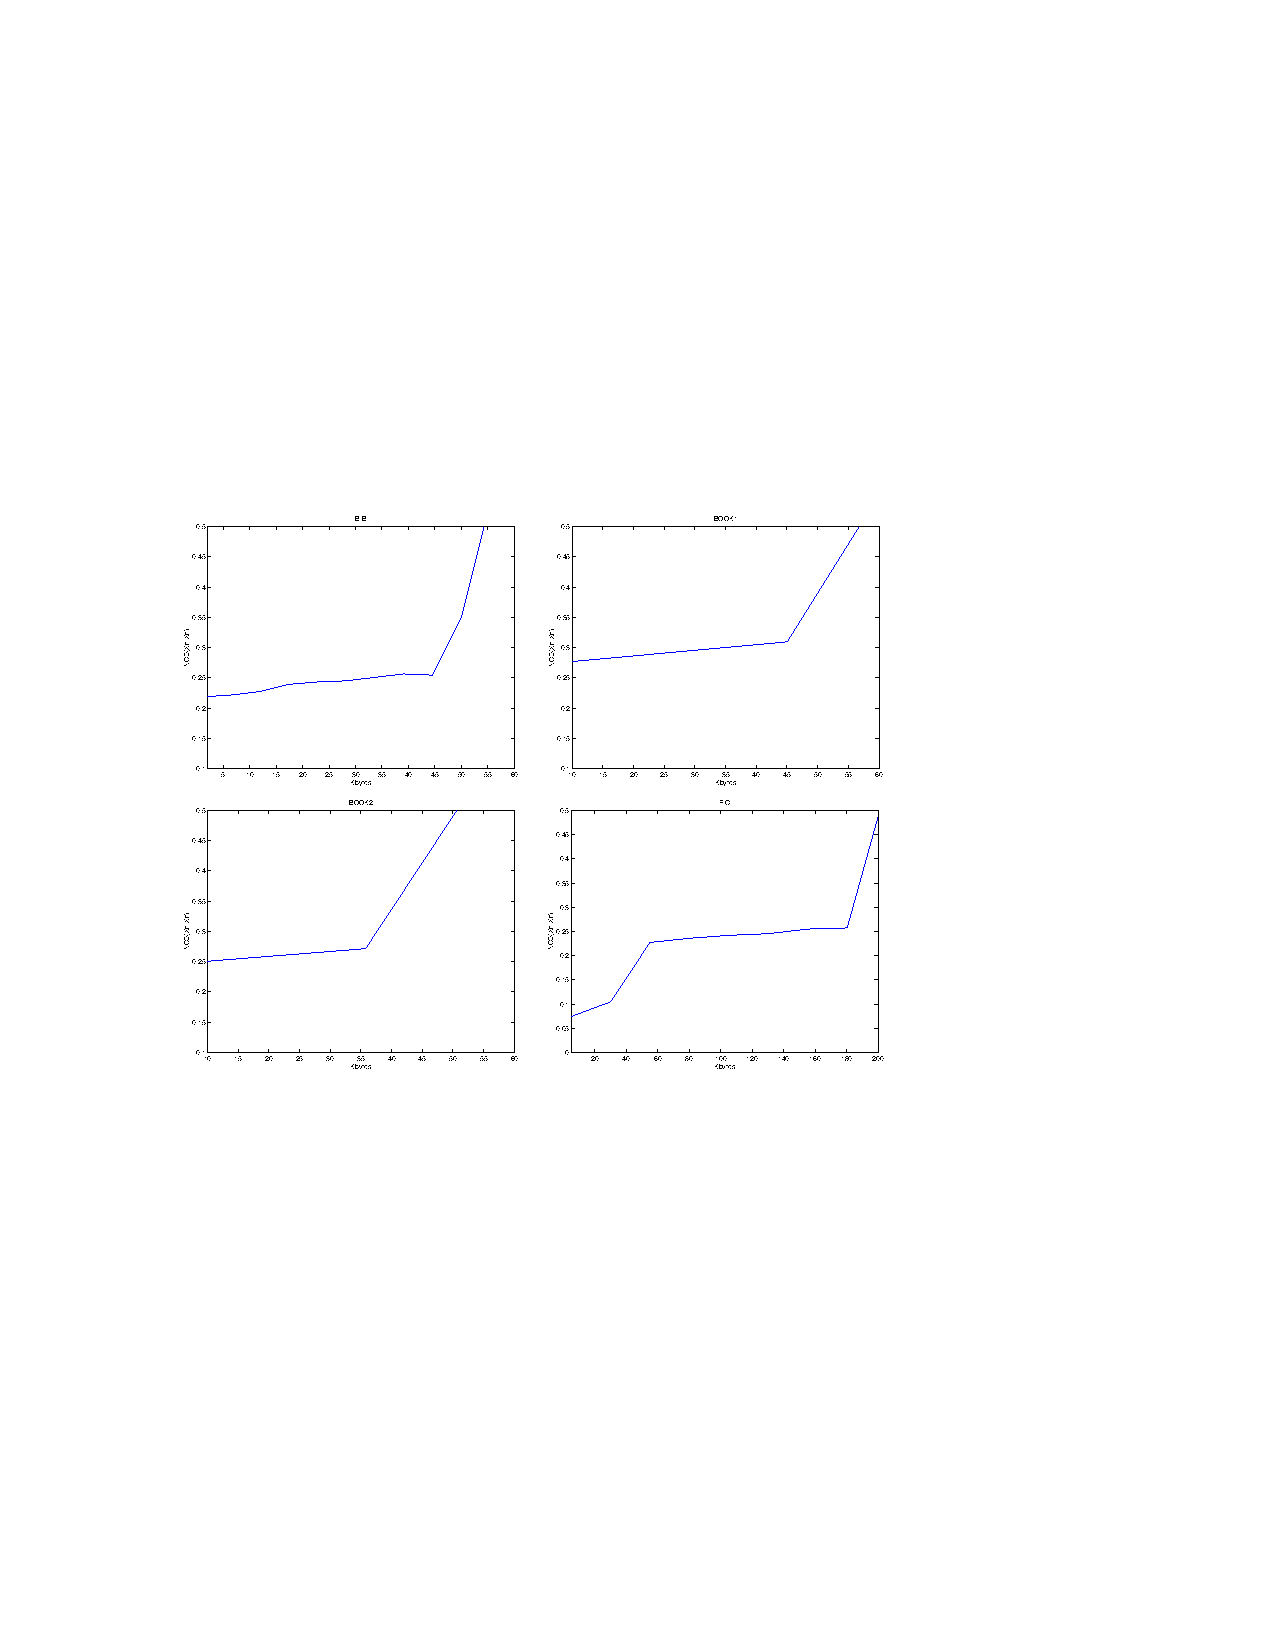
\includegraphics{img/bzip2-fast}
      \end{center}
      \caption{Normalisoidut pakkausetäisyydet ensimmäisestä $n$ tavusta, neljälle tiedostolle Calgary Corpus -kokoelmasta, käyttäen \emph{bzip2} pakkaajaa asetuksella `--fast' \cite{cebrian2005common}}
      \label{fig:bzip2-fast}
    \end{figure}
    \begin{figure}[t]
      \begin{center}
        \immediate\write18{pdfcrop img/gzip-best}
      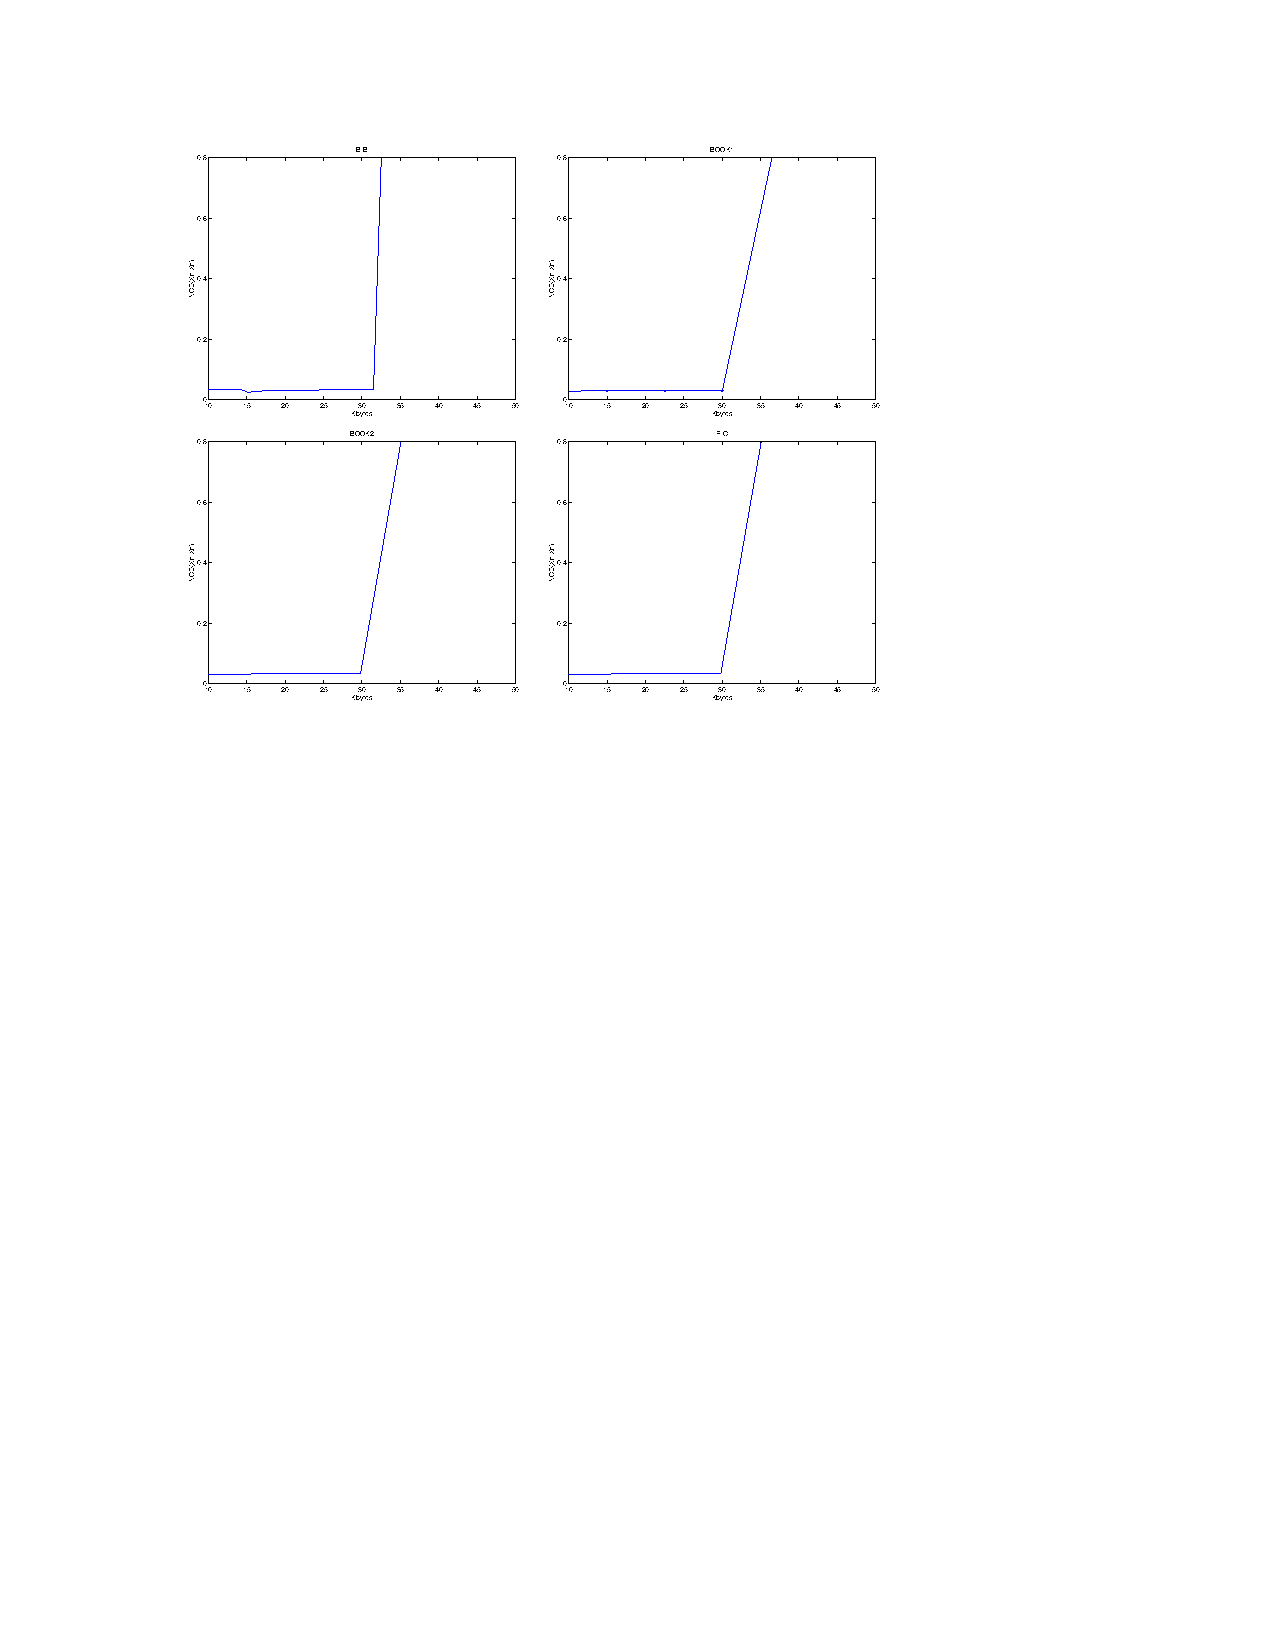
\includegraphics{img/gzip-best}

      \end{center}
      \caption{Normalisoidut pakkausetäisyydet ensimmäisestä $n$ tavusta, neljälle tiedostolle Calgary Corpus -kokoelmasta, käyttäen \emph{gzip} pakkaajaa asetuksella `--best' \cite{cebrian2005common}}
      \label{fig:gzip-best}
    \end{figure}
    \begin{figure}[t]
      \begin{center}
        \immediate\write18{pdfcrop img/ppmz}
      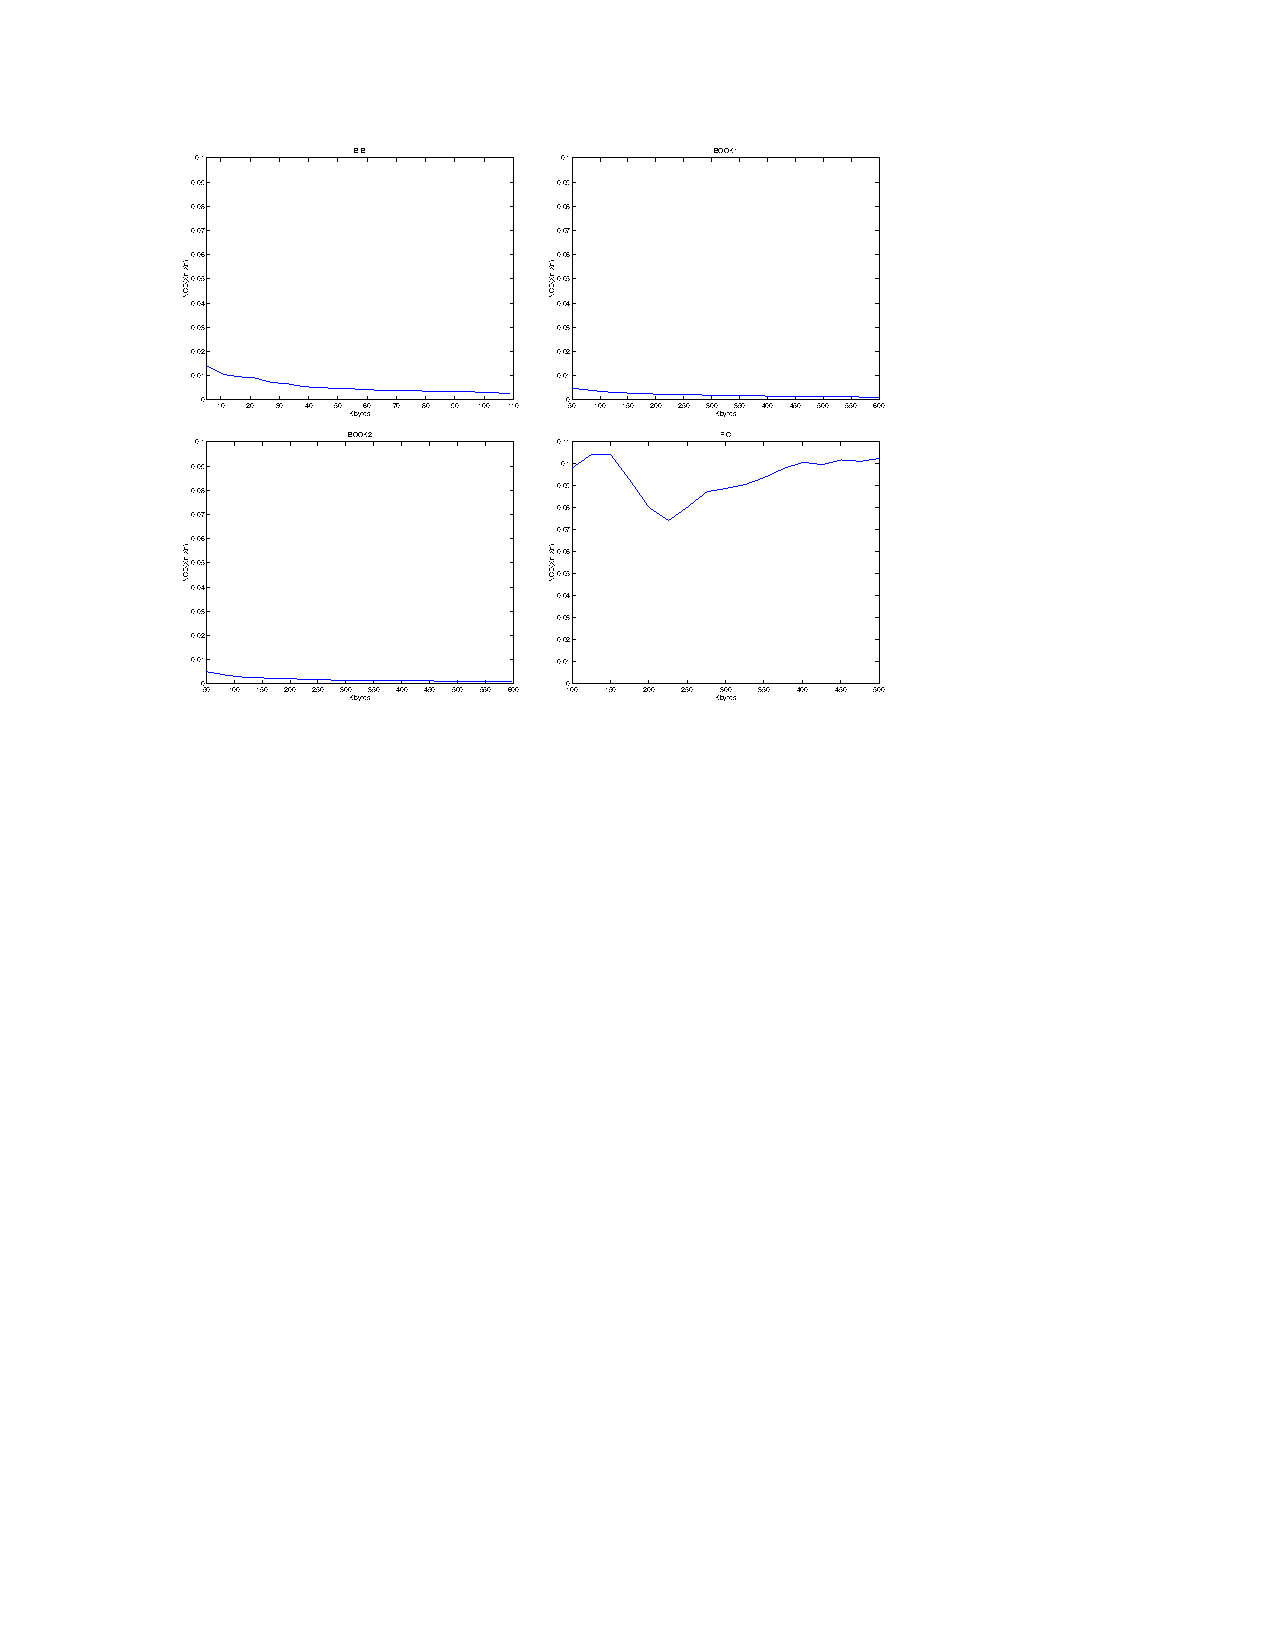
\includegraphics{img/ppmz}
      \end{center}
      \caption{Normalisoidut pakkausetäisyydet ensimmäisestä $n$ tavusta, neljälle tiedostolle Calgary Corpus -kokoelmasta, käyttäen \emph{PPMZ} pakkaajaa \cite{cebrian2005common}}
      \label{fig:ppmz}
    \end{figure}
    \iffalse
      TODO: This paper shows that the compressors used to compute the normalized compression distance are not idempotent in some cases, being strongly skewed with the size of the objects and window size, and therefore causing a deviation in the identity property of the distance if we don’t take care that the objects to be compressed fit the windows. The relationship underlying the precision of the distance and the size of the objects has been analyzed for several well-known compressors, and specially in depth for three cases, bzip2, gzip and PPMZ which are examples of the three main types of compressors: block-sorting, Lempel-Ziv, and statistic.
    \fi
      NCD vaikuttaa tuottavan vaikuttavia tuloksia klusteroinnissa, mutta tulokset ovat hyvin vahvasti riippuvaisia käytetyn pakkaajan ominaisuuksista.
      Suosittuja pakkaajia \emph{bzip2}, \emph{gzip} ja \emph{PPMZ} vertailtiin NCD:n kanssa \cite{cebrian2005common}, selvittääksen mitä heikkouksia, jos mitään, näillä on.


      Vertailussa käytettiin Cilibrasin toteuttamaa CompLearn -työkalua \cite{complearn}, josta löytyy bzip2 ja gzip pakkaajat. Aineistona käytettiin tunnettua Calgary Corpus -kokoelmaa \cite{calgarycorpus}, joka on 18 tiedoston kokoelma jolla mitataan pakkausalgoritmien suorituskykyä. Kokoelmassa on 9 eri tyyppistä tiedostoa, jotta voidaan saada laaja näkemys pakkaussalgoritmin toiminnasta. Mukana muun muassa on kuva, kirjoja, artikkeleita, lähdekoodia ja tietokoneohjelmia.

      Kaikkia vertailun objekteja käsitellään merkkijonoinen, jotka koostuvat tavuista. Jotta voitiin todeta pakkaajan idempotenssin (\ref{idempotency}) pätevyys, kaikki objektit vertailtiin itsensä kanssa.

      Näistä vertailtiin ensiksi bzip2 pakkaajaa, jolle pitää määrittää lohkon koko

    \begin{itemize}
      \item bzip2 ja lohkon koko
      \item gzip, liukuva ikkuna ja eteenpäinkatselikkuna
      \item ppmz, hidasta mutta tehokasta, koska ei mitään rajoitteita materiaalin koolle
      \item Lopputulos, jos pyritään klusteroimaan NCD:llä pitäisi aina käyttää PPMZ:taa tai vastaavaa pakkaajaa joka ei rajoita tiedostonkokoa
    \end{itemize}



  % subsection pakkaajan_valinta (end)
% section algoritmin_ongelmat_ja_ominaisuudet (end)

\section{Muita samankaltaisuuden metriikoita} % (fold)
\label{sec:muita_samankaltaisuuden_metriikoita}
  Tässä kappaleessa esitellään muita samankaltaisuuden metriikoita, kuten Google samankaltaisuusetäisyys \engl{Google Similarity Distance}
  \subsection{Google samankaltaisuusetäisyys} % (fold)
  \label{sub:google_similarity_distance}

    % TODO: meaningful
    % TODO: aggregoidun

    Internetin kasvu on houkutellut miljoonia käyttäjiä luomaan miljardeja internetsivuja, jotka ovat keskiarvoltaan heikkolaatuisia. Suunnaton tiedon määrä miltei mistä tahansa aiheesta tekee siitä mahdollisen, että ääripäät kumoutuvat ja täten surin osa tai keskiverto on meaningful heikkolaatuisena approksimaationa. Täten kehitettiin yleinen metodi hyödyntämään tätä matalalaatuista tietoa, jota saa ilmaiseksi Internetistä. Tämä tietovarasto on kaikille käytettävissä käyttäen mitä tahansa hakukonetta, joka pystyy palauttamaan aggregoidun sivulukumäärä arvion, kuten Google.

    Google samankaltaisuusetäisyys (\emph{GSD}) on hyvin vahvasti verrattavissa Normalisoituun pakkausetäisyyteen \ref{sub:normalisoitu_pakkauset_isyys}, sillä kummatkin algoritmit perustuvat samoihin tekniikoihin, kuten Kolmogorv-kompleksisuuteen (\ref{sub:kolmogorov_kompleksisuus}) ja Normalisoituun informaatioetäisyyteen (\ref{sub:normalisoitu_informaatioet_isyys}).
    Eroavaisuuksia esiintyy siinä, että mitä nämä kaksi algoritmiä käyttävät samankaltaisuuden arvioimiseksi.
    Siinä missä NCD pakkaa ja vertaa sisältöä toisiinsa, niin GSD vertaa asioitten nimiä esiintymistiheyteen.

    \subsubsection{Käytännön esimerkki} % (fold)
    \label{ssub:k_yt_nn_n_esimerkki}
      GSD muodostetaan siten että haetaan ensiksi yhdellä hakutermillä, sitten toisella ja sen jälkeen kummallakin yhdessä.
      Hakujen lukumäärät vertaillaan keskenään ja normalisoidaan ja tästä saadaan samankaltaisuusetäisyys.

      Paperissa \cite{cilibrasi2007google} käytettiin hakusanoja ``horse'' ja ``rider'' esimerkkinä ja vuonna 2007 tuloksena oli $NGD(horse, rider) \approx 0.443$.
      Toistimme kyseisen haun 13.11.2013 ja tuloksena oli $NGD(horse, rider) \approx 0.233$.
      Arvojen suurta eroa on vaikea selvittää ilman laajempaa tutkimusta, mutta vaikuttavia tekoja on internetin kasvu, sekä epäselvyys mikä on tarkka lukumäärä Googlen indeksoituja sivuja.

    % subsubsection k_yt_nn_n_esimerkki (end)

    \subsubsection{Theory of Googling for similarity} % (fold) % TODO: Otsikko
    \label{ssub:theory_of_googling_for_similarity}

    % subsubsection theory_of_googling_for_similarity (end)



  % subsection google_similarity_distance (end)
% section muita_samankaltaisuuden_metriikoita (end)

\section{``Loppukaneetti''} % (fold)
\label{sec:loppukaneetti}

% TODO: Yhteenveto ongelmissa ja ominaisuuksista
% TODO: Viittaus johonkin muuhun klusterointiin

% section loppukaneetti (end)
\pagebreak
% --- References ---
%
% bibtex is used to generate the bibliography. The babplain style
% will generate numeric references (e.g. [1]) appropriate for theoretical
% computer science. If you need alphanumeric references (e.g [Tur90]), use
%
\bibliographystyle{babalpha-lf}
%
% instead.

% \bibliographystyle{babplain-lf}
\bibliography{references-fi}


% --- Appendices ---

% uncomment the following

% \newpage
% \appendix
%
% \section{Esimerkkiliite}

\end{document}
